\section{Positivity-Preserving IMEX Schemes}
\label{sec:imex}

In this section we discuss the class of IMEX schemes we consider for the realizability-preserving DG-IMEX method for the two-moment model developed in Section~\ref{sec:realizableDGIMEX} (see also \ref{app:butcherTables} for additional details).  
The semi-discretization of the moment equations with the DG method given by Eq.~\eqref{eq:semidiscreteDG} results in a system of ordinary differential equations (ODEs) in each element of the form
\begin{equation}
  \dot{\vect{u}}
  =\vect{\cT}(\vect{u})+\f{1}{\tau}\,\vect{\cQ}(\vect{u}),
  \label{eq:ode}
\end{equation}
where $\vect{u}$ are the degrees of freedom evolved with the DG method; i.e., for a test space spanned by $\{\phi_{i}(\vect{x})\}_{i=1}^{N}\in\bbV^{k}$, we let
\begin{equation}
  \vect{u}=\f{1}{|\bK|}\Big(\,\int_{\bK}\vect{\cM}_{h}\,\phi_{1}\,d\vect{x},\int_{\bK}\vect{\cM}_{h}\,\phi_{2}\,d\vect{x},\ldots,\int_{\bK}\vect{\cM}_{h}\,\phi_{N}\,d\vect{x}\,\Big)^{T}.
\end{equation}
Thus, for $\phi_{1}=1$, the first components of $\vect{u}$ are the cell averaged moments.  
In Eq.~\eqref{eq:ode}, the transport operator $\vect{\cT}$ is due to the second and third term on the left-hand side of Eq.~\eqref{eq:semidiscreteDG}, while the collision operator $\vect{\cQ}$ is due to the right-hand side of Eq.~\eqref{eq:semidiscreteDG}.  

\subsection{Second-Order Accurate, Positivity-Preserving IMEX Schemes}

In the applications of interest to us, collisions with a background induce stiffness ($\tau\ll1$) in regions of the computational domain and must be treated with implicit methods, while we can resolve the time scales induced by the transport term, which we then can treat with explicit methods.  
This motivates the use of IMEX methods \cite{ascher_etal_1997,pareschiRusso_2005}.  
Furthermore, we would like to employ IMEX schemes that preserve realizability of the moments --- subject only to a time step governed by the explicit transport operator, and comparable to the time step required for numerical stability of the explicit scheme.  
(The realizability-preserving and positivity-preserving properties of an IMEX scheme are intimately related, and we use the two phrases interchangeably.)  
Until recently, high-order (second or higher order temporal accuracy) positivity-preserving IMEX methods with time step restrictions solely due to the transport operator were not known.  
Chertock et al. \cite{chertock_etal_2015} presented second-order accurate IMEX schemes with a correction step.  
However, the correction step in \cite{chertock_etal_2015} involves both the transport and collision operators, and we have found that realizability is then subject to a time step restriction that depends on $\tau$, which may become too restrictive for stiff problems.  
More recently, Hu et al. \cite{hu_etal_2018}, presented similar IMEX schemes for problems involving BGK-type collision operators, but with a correction step that does not include the transport operator.  
In this case, positivity is only subject to time step restrictions stemming from the transport operator, which is more attractive for our target application.  
These second-order accurate, $s$-stage IMEX schemes take the following form \cite{hu_etal_2018}
\begin{align}
  \vect{u}^{(i)}
  &=\vect{u}^{n}
  +\dt\sum_{j=1}^{i-1}\tilde{a}_{ij}\,\vect{\cT}(\vect{u}^{(j)})
  +\dt\sum_{j=1}^{i}a_{ij}\,\f{1}{\tau}\,\vect{\cQ}(\vect{u}^{(j)}),
  \quad i=1,\ldots,s, \label{imexStages} \\
  \tilde{\vect{u}}^{n+1}
  &=\vect{u}^{n}
  +\dt\sum_{i=1}^{s}\tilde{w}_{i}\,\vect{\cT}(\vect{u}^{(i)})
  +\dt\sum_{i=1}^{s}w_{i}\,\f{1}{\tau}\,\vect{\cQ}(\vect{u}^{(i)}), \label{imexIntermediate} \\
  \vect{u}^{n+1}
  &=\tilde{\vect{u}}^{n+1}-\alpha\,\dt^{2}\,\f{1}{\tau^{2}}\,\vect{\cQ}'(\vect{u}^{*})\,\vect{\cQ}(\vect{u}^{n+1}), \label{eq:imexCorrection}
\end{align}
where, as in standard IMEX schemes, $(\tilde{a}_{ij})$ and $(a_{ij})$, components of $s\times s$ matrices $\tilde{A}$ and $A$, respectively, and the vectors $\tilde{\vect{w}}=(\tilde{w}_{1},\ldots,\tilde{w}_{s})^{T}$ and $\vect{w}=(w_{1},\ldots,w_{s})^{T}$ must satisfy certain order conditions \cite{pareschiRusso_2005}.  
The coefficient in the correction step is positive, $\alpha>0$, and $\vect{\cQ}'$ is the Fr{\'e}chet derivative of the collision term evaluated at $\vect{u}^{*}$.  
For second-order accuracy, $\vect{\cQ}'$ can be evaluated using any of the stage values ($\vect{u}^{n}$, $\vect{u}^{(i)}$, or $\tilde{\vect{u}}^{n+1}$).  
For second-order temporal accuracy, the order conditions for the IMEX scheme in Eqs.~\eqref{imexStages}-\eqref{eq:imexCorrection} are
\begin{equation}
  \sum_{i=1}^{s}\tilde{w}_{i}=\sum_{i=1}^{s}w_{i}=1,
  \label{orderConditions1}
\end{equation}
and
\begin{equation}
  \sum_{i=1}^{s}\tilde{w}_{i}\,\tilde{c}_{i}
  =\sum_{i=1}^{s}\tilde{w}_{i}\,c_{i}
  =\sum_{i=1}^{s}w_{i}\,\tilde{c}_{i}
  =\sum_{i=1}^{s}w_{i}\,c_{i}-\alpha=\f{1}{2}, 
  \label{orderConditions2}
\end{equation}
where $\tilde{c}_{i}$ and $c_{i}$ are given in \ref{app:butcherTables}.  
For globally stiffly accurate (GSA) IMEX schemes, $\tilde{w}_{i}=\tilde{a}_{si}$ and $w_{i}=a_{si}$ for $i=1,\ldots,s$, so that $\tilde{\vect{u}}^{n+1}=\vect{u}^{(s)}$ \cite{ascher_etal_1997}.  
This property is beneficial for very stiff problems, and also simplifies the proof of the realizability-preserving property of the IMEX scheme since it eliminates the assembly step in Eq.~\eqref{imexIntermediate}.  

To prove the positivity-preserving property of the IMEX scheme, Hu et al. \cite{hu_etal_2018} rewrite the stage values in Eq.~\eqref{imexStages} in the following form
\begin{equation}
  \vect{u}^{(i)}
  =\sum_{j=0}^{i-1}c_{ij}\Big[\,\vect{u}^{(j)}+\hat{c}_{ij}\,\dt\,\vect{\cT}(\vect{u}^{(j)})\,\Big]
  +a_{ii}\,\dt\,\f{1}{\tau}\,\vect{\cQ}(\vect{u}^{(i)}),\quad i=1,\ldots,s,
  \label{eq:imexStagesRewrite}
\end{equation}
where $c_{ij}$, and $\hat{c}_{ij}=\tilde{c}_{ij}/c_{ij}$ are computed from $\tilde{a}_{ij}$ and $a_{ij}$ (see \ref{app:butcherTables}).  
In Eq.~\eqref{eq:imexStagesRewrite}, $\vect{u}^{(0)}=\vect{u}^{n}$.  
Two types of IMEX schemes are considered: \emph{type~A} \cite{pareschiRusso_2005,dimarcoPareschi2013} and \emph{type~ARS} \cite{ascher_etal_1997}.  
For IMEX schemes of type~A, the matrix $A$ is invertible.  
For IMEX schemes of type~ARS, the matrix $A$ can be written as
\[\left( 
   \begin{matrix} 
       0 & 0 \\ 
       0 & \hat{A}
   \end{matrix}
\right)\]
where $\hat{A}$ is invertible.  
In writing the stages in the IMEX scheme in the general form given by Eq.~\eqref{eq:imexStagesRewrite}, it should be noted that $\tilde{c}_{i0}=0$ for IMEX schemes of Type~A, and $c_{i1}=\tilde{c}_{i1}=0$ for IMEX schemes of Type~ARS \cite{hu_etal_2018}.  
For type A schemes, the positivity-preserving property follows from requiring $a_{ii}>0$ and $c_{i0}\ge0$ for $i=1,\ldots,s$, and $c_{ij},\tilde{c}_{ij}\ge0$, for $i=2,\ldots,s$, $j=1,\ldots,s-1$.  
For type ARS schemes, positivity follows from requiring $a_{ii}>0$ and $c_{i0},\tilde{c}_{i0}\ge0$ for $i=2,\ldots,s$, and $c_{ij},\tilde{c}_{ij}\ge0$ for $i=3,\ldots,s$, $j=2,\ldots,i-1$.  
Such coefficients were given in \cite{hu_etal_2018} for GSA schemes of type A with $s=3$ and type ARS with $s=4$.  
(It was also proven that $s=3$ and $s=4$ are the necessary number of stages needed for GSA second-order positivity-preserving IMEX schemes of type A and type ARS, respectively.)  

Importantly, the coefficients $c_{ij}$ in Eq.~\eqref{eq:imexStagesRewrite} satisfy $\sum_{j=0}^{i-1}c_{ij}=1$, which implies the so-called Shu-Osher form of the explicit part \cite{shuOsher_1988}.  
If the expression inside the square brackets in Eq.~\eqref{eq:imexStagesRewrite} --- which is in the form of a forward Euler update with time step $\hat{c}_{ij}\,\dt$ --- is positive for all $i=1,\ldots,s$, $j=0,\ldots,i-1$, positivity of the entire sum on the right-hand side of Eq.~\eqref{eq:imexStagesRewrite} follows from convexity arguments.  
Thus, if the explicit update with the transport operator is positive for a time step $\dt_{\mbox{\tiny Ex}}$, the IMEX scheme is positivity-preserving for a time step $\dt\le c_{\mbox{\tiny Sch}}\,\dt_{\mbox{\tiny Ex}}$, where
\begin{equation}
  c_{\mbox{\tiny Sch}}=\min_{\substack{i = 2,\ldots,s \\ 
       j = 1,\ldots,i-1}}\,\f{1}{\hat{c}_{ij}} \quad \text{(Type A)}, \quad  c_{\mbox{\tiny Sch}}=\min_{\substack{i = 2,\ldots,s \\ 
              j = 0,2,\ldots,i-1}}\,\f{1}{\hat{c}_{ij}} \quad \text{(Type ARS)}.
  \label{eq:imexCFL}
\end{equation}
It is desirable to make $c_{\mbox{\tiny Sch}}$ as large (close to $1$) as possible.  
Note that positivity of $\vect{u}^{(i)}$ also requires the implicit solve (equivalent to implicit Euler) to preserve positivity.  
In \cite{hu_etal_2018}, Hu et al. provide examples of GSA, positivity-preserving IMEX schemes of type A (see scheme PA2 in \ref{app:butcherTables}) and type ARS.  
In \ref{app:butcherTables}, we provide another example of a GSA, positivity-preserving IMEX scheme of type A (scheme PA2+), with a larger $c_{\mbox{\tiny Sch}}$ (a factor of about $1.7$ larger).  

\subsection{Positivity-Preserving, Diffusion Accurate IMEX Schemes}

Unfortunately, the correction step in Eq.~\eqref{eq:imexCorrection} deteriorates the accuracy of the IMEX scheme when applied to the moment equations in the diffusion limit ($\xi=0$, $\tau\ll 1$), where $\vect{\cK}\approx\f{1}{3}\,\cJ\,\vect{I}$.  
In the diffusion limit, to leading order in $\tau$, we then have $\vect{\cH}\approx-\f{1}{3}\,\tau\,\nabla\cJ$, which is due to a balance between the transport term and the collision term in the equation for the particle flux $\vect{\cH}$.  
The absence of the transport operator in the correction step, destroys this balance.  
We demonstrate the inferior performance of IMEX schemes with the correction step given by Eq.~\eqref{eq:imexCorrection} in the diffusion limit in Section~\ref{sec:smoothProblems}.  
We have also implemented and tested one of the IMEX schemes in Chertock et al. \cite{chertock_etal_2015}, where the transport operator is included in the correction step, and found it to perform very well in the diffusion limit.  
However, we have not been able to prove the realizability-preserving property with this approach without invoking a too severe time step restriction.  
We therefore proceed to design positivity-preserving IMEX schemes, without the correction step, that perform better in the diffusion limit.  
We limit the scope to IMEX schemes of type~ARS.  
(It can be shown that IMEX schemes of type~A conforming to Definition~\ref{def:PD-IMEX} below do not exist; cf. \ref{app:noTypeA}.)

To this end we take a heuristic approach and define the vectors 
\begin{equation}
  \vec{\cJ}=(\cJ^{(1)},\ldots,\cJ^{(s)})^{T}
  \quad\text{and}\quad
  \vec{\vect{\cH}}=(\vect{\cH}^{(1)},\ldots,\vect{\cH}^{(s)})^{T}.  
\end{equation}
In the context of IMEX schemes, the diffusion limit balance implies that the relation $A\,\vec{\vect{\cH}}=-\f{1}{3}\,\tau\,\tilde{A}\,\nabla\vec{\cJ}$ should hold to relate the stage values in Eq.~\eqref{imexStages}.  
Define the inverse of the implicit coefficient matrix for IMEX schemes of type~ARS as
\begin{equation*}
    A^{-1}
    =\left(
        \begin{matrix}
          0 & 0 \\ 
          0 & \hat{A}^{-1}
        \end{matrix}
      \right).
\end{equation*}
For the stages $i=1,\ldots,s$ we have
\begin{equation}
  \vect{\cH}^{(i)}=-\f{1}{3}\,\tau\,\vect{e}_{i}^{T}A^{-1}\tilde{A}\,\vect{e}\,\nabla\cJ^{n}+\cO(\dt\,\tau),
\end{equation}
where $\vect{e}_{i}$ is the $i$th column of the $s\times s$ identity matrix and $\vect{e}=(1,\ldots,1)^{T}$.  
Thus, for $\vect{\cH}^{(i)}$ to be accurate in the diffusion limit, we require the IMEX coefficients to satisfy
\begin{equation}
  \vect{e}_{i}^{T}A^{-1}\tilde{A}\,\vect{e} = 1, \quad i=2,\ldots,s.
  \label{eq:diffusionCondition}
\end{equation}
(The case $i=1$ is trivial and does not place any constraints on the IMEX coefficients.)  
Then, for the particle number equation we have
\begin{equation}
  \f{\cJ^{(s)}-\cJ^{n}}{\dt}
  =-\tilde{\vect{w}}^{T}(\nabla\cdot\vec{\vect{\cH}})
  \approx\f{1}{3}\tau\,\nabla^{2}\cJ^{n}, 
\end{equation}
which approximates a diffusion equation with the correct diffusion coefficient $\tau/3$.  
Unfortunately, the ``diffusion limit requirement" in Eq.~\eqref{eq:diffusionCondition}, together with the order conditions given by Eqs.~\eqref{orderConditions1} and \eqref{orderConditions2} (with $\alpha=0$), and the positivity conditions on $c_{ij}$ and $\tilde{c}_{ij}$, result in too many constraints.  
(It was shown in \cite{hu_etal_2018} --- without the diffusion limit requirement --- that the minimum number of stages for positivity-preserving IMEX schemes of type~ARS is four.)  
We are also concerned about increasing the number of stages, and thereby the number of implicit solves, since the implicit solve will dominate the computational cost of the IMEX scheme with more realistic collision operators (e.g., inelastic scattering).  
To reduce the number of constraints, and accommodate accuracy in the diffusion limit, we relax the requirement of overall second-order accuracy of the IMEX scheme.  
Instead, we only require the scheme to be second-order accurate in the streaming limit ($\vect{\cQ}=0$).  
This gives the order conditions
\begin{equation}
  \sum_{i=1}^{s}\tilde{w}_{i}=1
  \quad\text{and}\quad
  \sum_{i=1}^{s}\tilde{w}_{i}\,\tilde{c}_{i}=\f{1}{2},
  \label{eq:orderConditionsEx}
\end{equation}
where the first condition (consistency condition) is required for first-order accuracy.  
We then seek to design IMEX schemes of Type~ARS conforming to the following working definition
\begin{define}
  Let PD-IMEX be a consistent, positivity-preserving, diffusion accurate, and low-stage GSA IMEX scheme satisfying the following properties
  \begin{itemize}
    \item Consistency of the implicit coefficients
    \begin{equation}
      \sum_{i=1}^{s}w_{i}=1.
      \label{eq:implicitConsistency}
    \end{equation}
    \item Second-order in the streaming limit; i.e., satisfies Eq.~\eqref{eq:orderConditionsEx}.
    \item Positivity-preserving (conditions given by \cite{hu_etal_2018}; with $c_{\mbox{\tiny Sch}}>0$).
    \item Well-behaved in the diffusion limit; i.e., satisfies Eq.~\eqref{eq:diffusionCondition}.
    \item Few stages ($s\le3$).
    \item Globally stiffly accurate (GSA)
    \begin{equation*}
      a_{si}=w_{i}\quad\text{and}\quad\tilde{a}_{si}=\tilde{w}_{i},\quad i=1,\ldots,s.
    \end{equation*}
  \end{itemize}
  \label{def:PD-IMEX}
\end{define}
Fortunately, IMEX schemes of type~ARS satisfying these properties are easy to find, and we provide an example with $s=3$ (two implicit solves) in \ref{app:butcherTables} (scheme PD-ARS; see \ref{app:PD-ARS} for details).  
In the streaming limit, this scheme is identical to the optimal second-order accurate strong-stability preserving Runge-Kutta method \cite{gottlieb_etal_2001}.  
It is also very similar to the scheme given in \cite{mcclarren_etal_2008} (see scheme PC2 in \ref{app:butcherTables}), which is also a GSA IMEX scheme of type ARS with $s=3$.  
Scheme PC2 is second-order in the streaming limit, has been demonstrated to work well in the diffusion limit \cite{mcclarren_etal_2008,radice_etal_2013}, and satisfies the positivity conditions, but $c_{\mbox{\tiny Sch}}=0$ (our primary motivation for finding an alternative).  
In Section~\ref{sec:numerical}, we show numerically that the accuracy of scheme PD-ARS is comparable to the accuracy of scheme PC2.  

\subsection{Absolute Stability}

Here we analyze the absolute stability of the proposed IMEX schemes, PA2+ and PD-ARS (given in \ref{app:butcherTables}), following \cite{hu_etal_2018}.  
As is commonly done, we do this in the context of the linear scalar equation
\begin{equation}
  \dot{u}=\lambda_{1}\,u+\lambda_{2}\,u,
  \label{eq:scalarODE}
\end{equation}
where $\lambda_{1}\in\mathbb{C}$ and real $\lambda_{2}\le0$.  
On the right-hand side of Eq.~\eqref{eq:scalarODE}, the first (oscillatory) term is treated explicitly, while the second (damping) term is treated implicitly.  
The IMEX schemes can then be written as $u^{n+1} =P(z_{1},z_{2})\,u^{n}$, where $P(z_{1},z_{2})$ is the amplification factor of the scheme, $z_{1}=\dt\,\lambda_{1} = x +iy$, and $z_{2} = \dt\,\lambda_{2} < 0$.  
Stability of the IMEX scheme requires $|P(z_1,z_2)|\leq 1$.  
The stability regions of PA2+ and PD-ARS are plotted in Figure~\ref{fig:AbsoluteStability}.  
As can be seen from the figures, the absolute stability region of both schemes increases with increasing $|z_{2}|$.  
For a given $|z_{2}|>0$, the stability region of PD-ARS is larger than that of PA2+.  
In the linear case, a time step that satisfies the absolute stability for the explicit part of the IMEX scheme ($|z_2| = 0$) fulfills the stability requirement for the IMEX scheme as whole ($|z_2| \geq 0$).  
This conclusion is valid for all PD-ARS schemes with $\epsilon\in [0,0.5)$.
\begin{figure}[h]
  \centering
  \begin{tabular}{cc}
    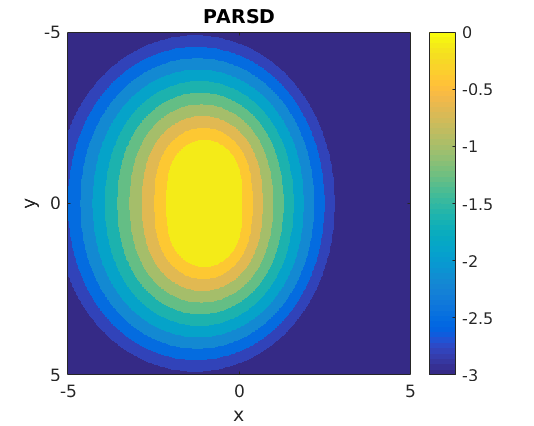
\includegraphics[width=0.5\textwidth]{figures/AbsoluteStabilityPARSD}
    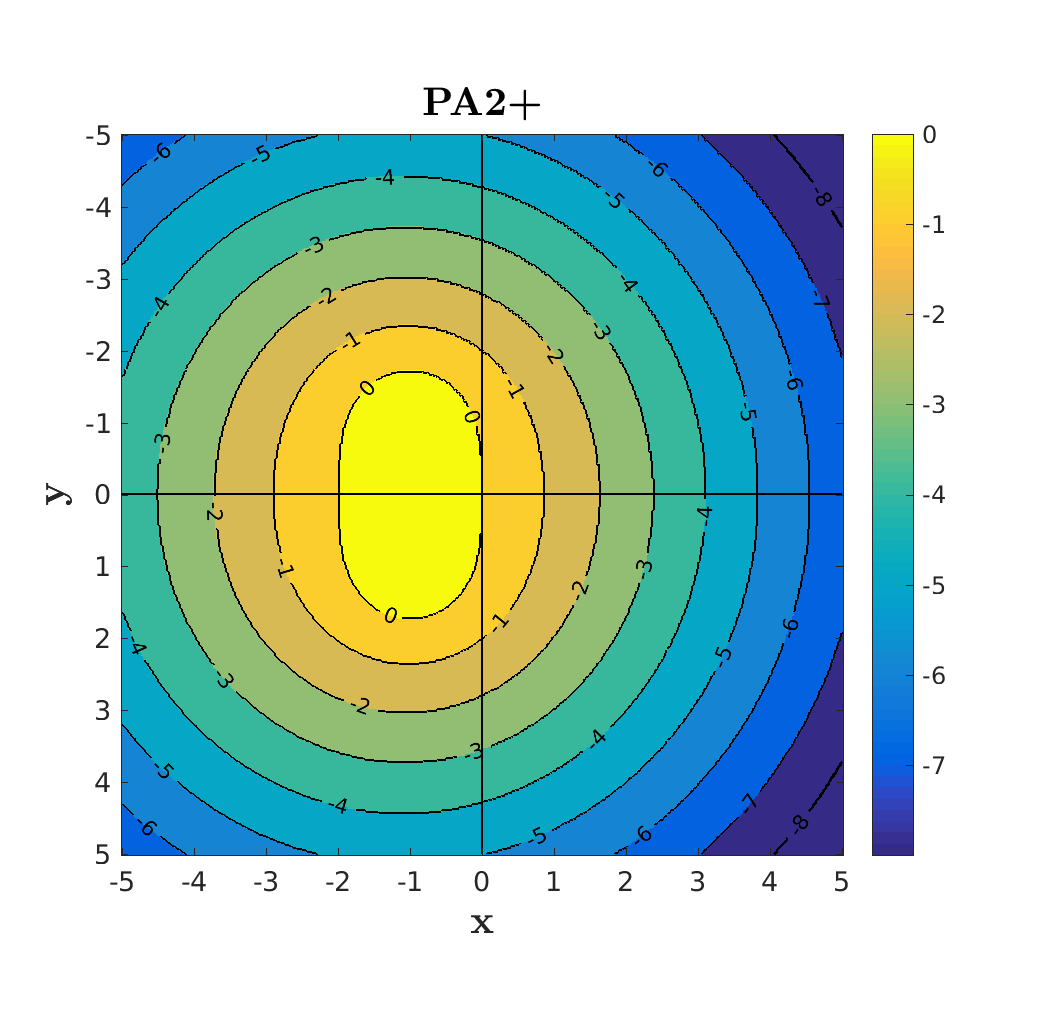
\includegraphics[width=0.5\textwidth]{figures/AbsoluteStabilityPA2+}
  \end{tabular}
   \caption{Boundary of the absolute stability region for different values of $z_2$ for PD-ARS with $\epsilon = 0.1$ (left panel) and PA2+ (right panel).}
  \label{fig:AbsoluteStability}
\end{figure}